
\documentclass[12pt]{article}
\usepackage{amsmath}
\usepackage{amssymb}
\usepackage{amsfonts}
\usepackage{mathrsfs}
\usepackage{bm}
\usepackage{indentfirst}
\setlength{\parindent}{0em}
\usepackage[margin=1in]{geometry}
\usepackage{graphicx}
\usepackage{setspace}
\doublespacing
\usepackage[flushleft]{threeparttable}
\usepackage{booktabs,caption}
\usepackage{float}
\usepackage{graphicx}

\usepackage{import}
\usepackage{xifthen}
\usepackage{pdfpages}
\usepackage{transparent}

\newcommand{\incfig}[1]{%
\def\svgwidth{\columnwidth}
\import{./figures/}{#1.pdf_tex}
}




\title{Summary}
\author{Yan Hao}
\date{Feb 28, 2021}


\begin{document}
\maketitle
\newpage




\section{Program Design}

This program is designed for predicting the price for each airbnb apartment.
The program will process in four steps.

First, drop all observations with missing values, extract
valuable variables, regroup prices to 7 groups, count how far was the last
review till now (last-review can be seen as an activity sign.), 
convert room\_type and neighborhood\_group to dummy variables, and then save
the clean dataset to full\_clean\_dataset.csv. 

Second, select a suitable model, among linear regression, lasso, and ridge,
to predict apartment price. Note, the data used for prediction contain dummy
variables of price range. The R square can be very low, around 10\%, if we
predict prices without price range column. And R square is around 60\% by adding
price range column. Since Lasso model performs slightly better than the other
two, the program saves the trained Lasso machine to a pickle file, called
price\_model.pickle.

Third, since price range is not included in the raw data, I need to train a 
machine to predict price range first. Since price range is categorical, the
potential models can be used are random forest (RF), logistic, and support vector
machine. The latter two models take much longer time to process the prediction, 
and they do not return a higher accuracy score. Hence, I did a grid search for
random forest by changing the number of trees and the maximum depth. 
The trend can be find in acc\_trend.png where x1 to x4 are the four accuracy score 
sequences, since I split the data to four groups using KFold. The vertical
axis presents the actual value of accuracy score. The horizontal axis presents the
indexing of the model. This indexing can help you to find detailed information
of RF with particular parameter settings in RF\_grid\_search\_results.csv.
From the trend in Figure 1, accuracy score of the second and the third splits are 
clearly higher than the first and the fourth split. Also, the accuracy scores are
seasonal fluctuate. The accuracy score goes down as the increase of maximum 
depth. Hence, I pick n\_estimators=16, max\_depth=11. This combination gives me
a better performance among others. Then the model is saved to 
PriceRange\_machine.pickle. 

Fourth, test the model. Now the program has saved the price\_model and the
PriceRange\_machine. I use the first 7000 observations to test the model.
In this step, the program firstly drop price and price range columns to form
a manually-made test data. Then it predicts price range by using PriceRange
machine, and merge this column with the data. And then the machine predicts price
using price model. The R square is about 0.2. This is not a good performance, but
it is higher than 0.1, which is the R square if we directly predict price without
price range. Note, if we can improve the performance of the prediction for
price range, the model can perform much better. 




\section{Problems of this program}

First, this program do not use information from latitude and longitude. I tried
to find the relation between price and location information. I have plotted each
apartment's latitude and longitude colored by different price range in 
Figure 2. It seems that apartment with same price range are clustered. But 
I do not find a method to describe it. 

Second, since I use pandas to convert dummy variables, if the exist data
does not have all price range, then the data used for price prediction will
have less column(s).




\newpage
\section{Figures}



\begin{figure}[H]
 \caption{Accuracy Rate Trend}
 \center{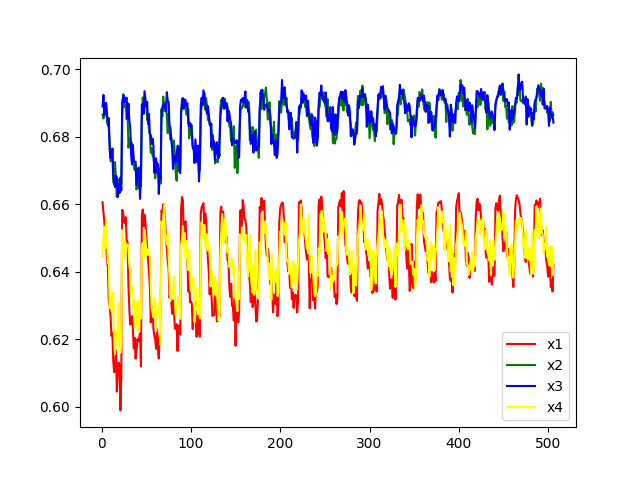
\includegraphics[scale = 1 ]  {figures/R2_trend.png}}
\end{figure}



\begin{figure}[H]
 \caption{Price and Location}
 \center{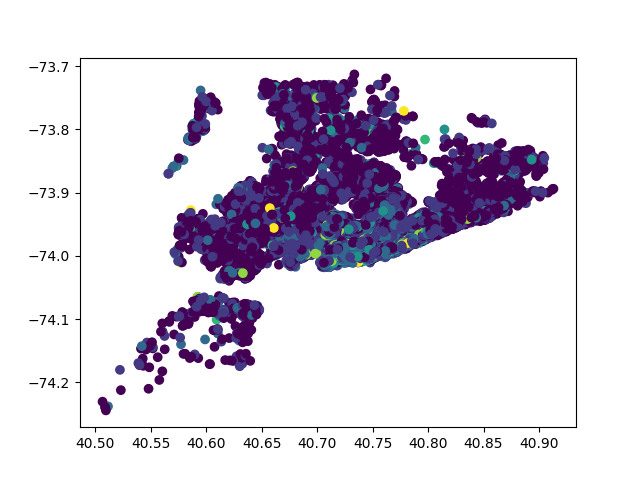
\includegraphics[scale = 1 ]  {figures/price_location.png}}
\end{figure}




















\end{document}

